% --------------------------------------------
%		CHAPTER 1
%---------------------------------------------

\chapter{Belle II and SuperKEKB (SKB) accelerator}

The first chapter introduces some of the main unexplained aspects of the Standard Model (SM), on which the Belle II physics program is founded. A short description of the SuperKEKB accelerator and the Belle II detector's structure is also presented and in conclusion some highlights on the current state of measurements.


%---------------------------------------------
%			1.1
%---------------------------------------------
\section{Physics program of the B-factories}

The SM is a physics theory that describes three of the fundamental forces involving elementary particles, which are strong, weak and electromagnetic interaction (with the exclusion of the gravitational one). It classifies all the elementary constituents of matter in 4 main groups: quark, leptons, bosons and Higgs, as shown in~\autoref{fig:sm}.


\begin{figure}[h]
\centering
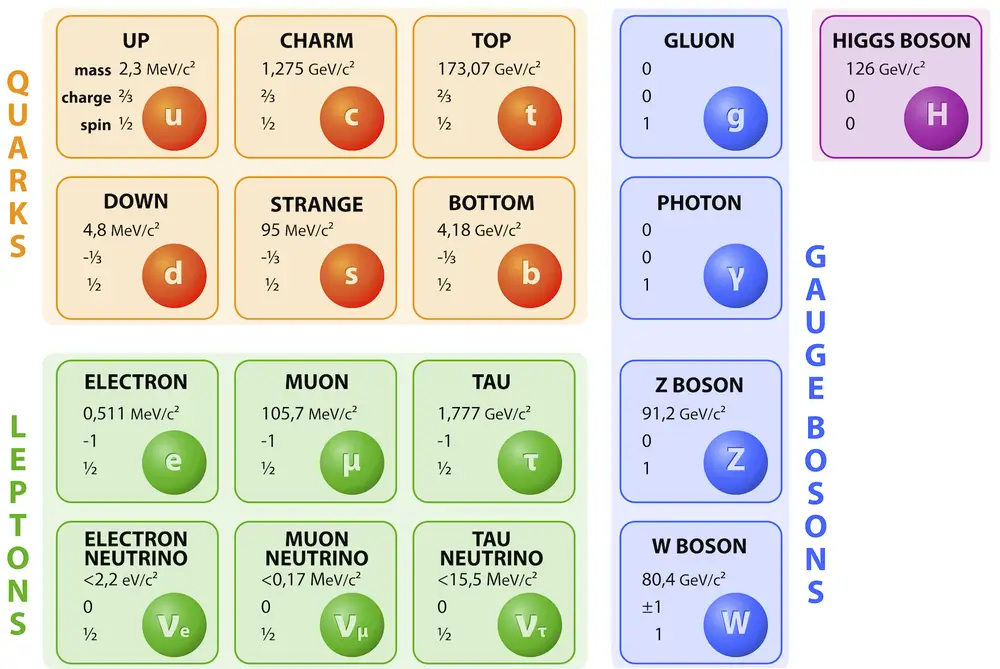
\includegraphics[scale=0.3]{SM}
\caption{Particle classification in the Standard Model.}
\label{fig:sm}
\end{figure}


%---------------------------------------------------------------------------------------


\subsection{Open questions in SM}


Despite the undeniable success of the SM in making predictions on physics phenomena, which have been experimentally verified with high precision over the years, there are many aspects of the Nature on which it is unable to give answers. Some of them are listed in the following.

\begin{itemize}
\item Three generations of quark and leptons have been discovered, but it is not known wheter they should be the only ones and the reasons behind their mass hierarchy.
\item Higgs mechanism is able to explain the cause of elementary particles' masses through spontaneous electro-weak symmetry breaking, but it is not clear wheter neutrinos could gain their masses through the interaction with the Higgs boson.
\item Another open question is the matter-antimatter asymmetry in the Universe. Even though Charge-Parity (CP) violation is necessary to explain its current state, the observed quantity is several orders of magnitude less than needed to explain the matter domination over antimatter, which allowed the evolution of the universe as we know it today.
\item In the SM the Cabibbo-Kobayashi-Maskawa (CKM) matrix describes the flavour-changing weak interaction through the mismatch between the quantum state of the freely propagating quarks. It could be parametrized by three mixing angles and a complex phase that is at the foundation of CP violation in the quark flavor sector. The fact that its elements are almost diagonal might suggest the existance of a new symmetry, that is unbroken at high energy (greater than the order of TeV).
\item Several astrophysical observations have been postulated the existance of dark matter, but its origin and nature have not been explained yet.
\end{itemize}

All these topics encourage the research of new particles and processes that could give reasonable answers.\\
At the energy frontier, experiments like the Large Hadron Collider (LHC) in Geneve are looking for new particles created from the proton-proton collision with a center mass energy up to 14 TeV.\\
At luminosity frontier instead, the hint of new particles and mechanisms is searched in precision measurements of suppressed reactions in flavour physics or in the deviations from SM. The discrepancies indeed, could be interpreted as a clue of new physics beyond SM. The last is the Belle II approach.\\


In particular the experiment investigates the CP violation in the B mesons system and it also searches for new physics evidences in the decays of B and D mesons, in $\tau$ leptons and in the dark matter sector (DM).

%-----------------------------------------------------------------------------------------

\subsection{Peculiarity of asymmetric B factories} \label{sec:vertex_decay}

The center of mass energy of Belle II experiment has its peak at the $\Upsilon(4S)$ resonance, such as $\sqrt{s}$ = 10.58 GeV, which decays almost instantaneously into two B mesons ($B^{0}$ - $\bar{B}^{0}$) in nearly 96\% of all cases. 

The main task of the VerteX Detector (VXD) is to reconstruct the production and decay vertices of the particles originated from the beam collisions. This aspect is crucial to perform time-dependent measurements, core of the Belle II physics program.

The choice of the asymmetric configuration of the beams relies precisely in the requirement to boost the mesons in order to measure their life-time, exploiting the information on the distance between their decay vertices. In fact in a beam symmetric situation, they would have been produced at rest, decaying roughly at the same point or in any case at undetectable distances. 
The investigation of CP violating processes instead, requires to measure the decay time difference of the two B mesons and its uncertainty is dominated by that of the decay vertex measurement (order of hundreds microns). Let us look at this in more details.\\

SuperKEKB collides an electrons beam of 7 GeV (High Energy Ring, HER) with a positrons beam of 4 GeV (Low Energy Ring, LER) and for this configuration results a Lorentz boost factor of the $\Upsilon(4S)$ of $(\beta\gamma)_{\Upsilon(4S)} \approx 0.28 $.

The same boost is also acquired by B mesons, because they are produced almost at rest ($m_{\Upsilon(4S)}$ - $m_{2B_{0}}\approx$ 19 MeV). Moreover knowing that $\tau_{B}\simeq $\num{1.5e-12} s and so c$\tau_{B}\simeq$ 450 $\mu$m, we can compute the average flight distance travelled before decaying:

\begin{equation}
\textit{l} = (\beta\gamma)_{\Upsilon(4S)}c\tau_{B} \approx 126 \mu m  
\end{equation} 

This value must be within the vertex detector sensitivity in order to distinguish the vertex decay and as consequence to make precision measurements of lifetimes, mixing parameters and CP violation. The six-layer VXD could determines the position of the vertices with a precision better than 100 $\mu$m, allowing to reconstruct secondary vertices, i.e. the decay position of the particles coming from B decays, and also from $\tau$ leptons and D mesons.

We want to take a closer look at the event kinematics (e.g.~\autoref{fig:decay_vertex}). The two B mesons are produced in an entangled quantum state, so from the decay products of the first it is possible to assign its flavor (for example $B^{0}$, identifyed as $B_{tag}^{0}$) and accordingly that of the second, which will be the opposite ($\bar{B}^{0}$, called $\bar{B}_{phys}^{0}$).

\begin{figure}[h!]
\centering
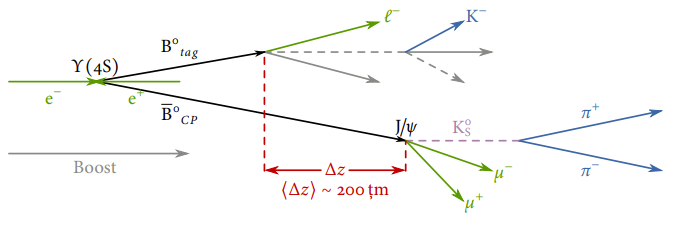
\includegraphics[scale=.9]{vertex_decay_1}
\caption{Example of the kinematics of the golden channel of Belle II experiment.}
\label{fig:decay_vertex}
\end{figure}

After this reconstruction, both B decay vertex positions in the longitudinal direction $\textit{z}_{1}$ and $\textit{z}_{2}$ are evaluated, in order to compute their difference:

\begin{equation}
\Delta \textit{z} = \textit{z}_{1} - \textit{z}_{2} = (\beta\gamma)_{\Upsilon(4S)}c\Delta t
\end{equation}

where $\Delta t$ is the proper time decay difference. 
Another important parameter used in the reconstruction is \textit{$d_{0}$}, which is the B decay vertex position from the primary vertex in the transverse plane.\\
Therefore this topology allows to transform a temporal information in a spatial one that we are able to measure. Without the boosted center of mass none of it could be possible, and this is an essential feature for an asymmetric B-factory. 


%---------------------------------------------
%			1.2
%---------------------------------------------
\section{SuperKEKB accelerator}

Belle II sensitivity in the precision measurements is feasible expecially thanks to the extraordinary performance of the SuperKEKB accelerator which host the (almost) hermetic detector. This complex facility is the result of efforts and efficient collaboration between the researches of KEK laboratory and all the international working groups that partecipate to the experiment.


\subsection{The facility}

SuperKEKB (\autoref{fig:superkekb}) is an asymmetric $e^{+}e^{-}$ collider with a circumference of 3 km and a center of mass energy peak equal to  $\sqrt{s}$ = 10.58 GeV, which corresponds to the mass of the $\Upsilon(4S)$ resonance.
Compared to its predecessor KEKB (which started its operation in 1998 and concluded it in 2010), the current accelerator has allowed to obtain the highest luminosity ever achieved, equal to \num{4.7e34} $cm^{-2}s^{-1}$ in July 2022. This target was possible using a new scheme to accelerate and collide the beams, the so called \textit{nano-beam scheme} (\autoref{sec:nano_beam}). 

Furthermore a new upgrade of the machine, still under study, will also include other interventions expecially to cope with higher background levels, in view of a future increase in luminosity.

\begin{figure}[h!]
\centering
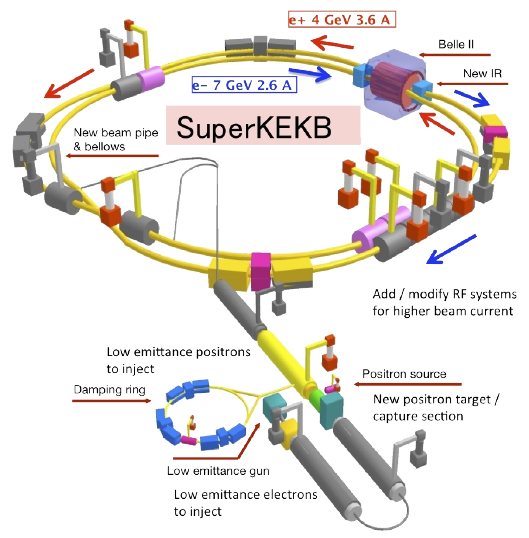
\includegraphics[scale=0.8]{SuperKEKB2}
\caption{SuperKEKB accelerator structure.}
\label{fig:superkekb}
\end{figure}


\bigskip

\textbf{Luminosity}\\

Istantaneous luminosity is one of the key parameters of any accelerator and it represents the interaction rate per unit of cross section between colliding particles. Reversing this equation is possible to obtain N, namely the number of the physical events produced in the interaction with a given luminosity:

\begin{equation}
L =\frac{1}{\sigma}\frac{dN}{dt}  \qquad   \Rightarrow \qquad  N = \int_{0}^{T} L\sigma dt
\end{equation}

where T is the duration of the experiment,  $\sigma$ the cross section of the physical process of interest. Although this is a raw information, as it does not consider other important factors that could influence the effective number of events produced, it becomes a significant starting point when one wants to study very rare processes such as Belle II.
Specifically luminosity is strictly dependent from both machine and beam parameters. With respect to this, it can be expressed as:

\begin{equation} \label{eq:luminosity_eq}
L = \frac{\gamma_{\pm}}{2er_{e}} \bigg(1 + \frac{\sigma_{y}^{*}}{\sigma_{x}^{*}} \bigg) \bigg(\frac{I_{\pm}\xi_{y\pm}}{\beta^{*}_{y}} \bigg) \bigg(\frac{R_{L}}{R_{\xi_{y\pm}}} \bigg)
\end{equation}

where ''$\pm$'' denotes respectively positrons and electrons beam, $\sigma_{x,y}^{*}$ is the beam size at the Interaction Point (IP) in the horizontal and vertical plane, $I$ is the beam current, $\beta_{y}^{*}$ the vertical beta function at the IP. $\xi_{y\pm}$ is the vertical beam parameter which include the horizontal beta function at the IP, the horizontal emittance, the bunch lenght and the crossing angle between the beams. $R_{L}$ and $R_{\xi_{y\pm}}$ are the reduction factors due to geometrical loss such as the hourglass effect and finite crossing.\\

As already mentioned, SuperKEKB holds the actual world record in luminosity (with $\beta^{*}_{y}$= 1.0 mm) and in the near future the target will be to reach \num{6e35} $cm^{-2} s^{-1}$ (by the 2030s), by increasing current beams and reducing their section at the IP, through the decrease of the betatron function down to $\beta^{*}_{y}= 0.3$ mm. But this process makes the beam-induced background grow a lot, risking deterioration and poor functioning of the detectors.

For these reasons the supervision of the beams background becomes crucial: right now it has been estimated that the background should remain accettable up to a luminosity value equal to \num{2.8e35} $cm^{-2} s^{-1}$ with $\beta^{*}_{y}$= 0.6 mm.
So the chance to achieve higher luminosity is closely related to an upgrade plan of both the whole detector and the accelerator.


\subsection{''Nano-beam'' scheme} \label{sec:nano_beam}

We have seen that the \textit{beta function} $\beta$ at the IP ($\beta^{*}$) is a decisive factor to define the luminosity. To be able to ramp the luminosity up, it is necessary to reduce the value of $\beta$ depending also, but not only, on the variation of the other machine parameters that appear in the~\autoref{eq:luminosity_eq}.

The mechanism used in SuperKEKB is called \textit{nano-beam scheme}, and it allowed to obtain luminosity 40 times greater than that of KEKB, managing to decrease of 1/20 the $\beta^{*}$.\\

This new scheme, originally designed by P. Raimondi, dictates that the beam bunches have to collide with sufficiently small $\sigma_{x}^{*}$ and at large angle. In case of SuperKEKB the latter is equal to 83 mrad at the IP (larger with respect to the crossing angle used in KEKB) with the beam size of 50 nm in the vertical direction and 100 $\mu$m in the horizontal direction (in~\autoref{fig:beam_scheme_comparison} a simplified representation of the differences).

This strategy also helps to reduce the \textit{hourglass effect}, which happens when the $\beta^{*}$ is comparable or smaller than the bunch lenght, causing a decrease in luminosity. As a matter of fact with larger crossing angle at the IP, the overlap lenght which is the effective bunch lenght, is much shorter than the bunch length along the beam axis. \\
%ARTICOLO A


\begin{figure}[h!]
\centering
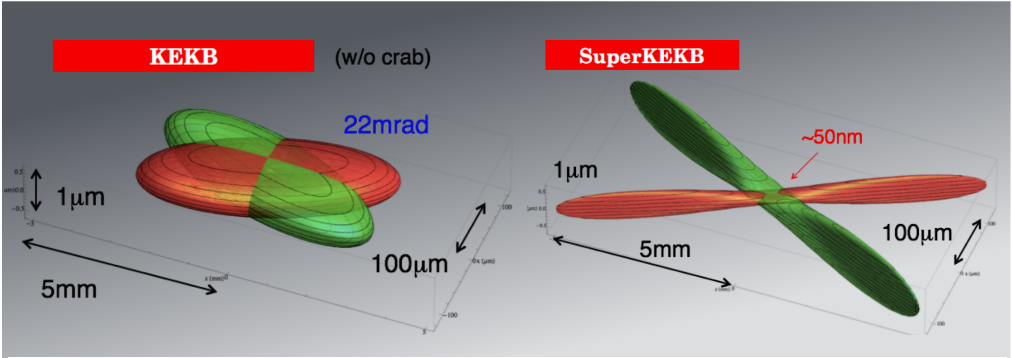
\includegraphics[scale=0.6]{nano_beam_scheme0}
\caption{Comparison between the beam schemes used in KEKB and SuperKEKB.}
\label{fig:beam_scheme_comparison}
\end{figure}

Using a crossing angle large enough has other positive implications on the operation of the accelerator and its further improvements, like allowing the placement of a new focusing system at the IP (which may require more space), considering a future redesign of the interaction region.

\begin{comment}
In~\autoref{fig:beampar} are reported the main machine parameters (default value) of the SuperKEKB accelerator.

%DA CONTROLLARE SE METTERE O MENO
\begin{figure}[h!]
\centering
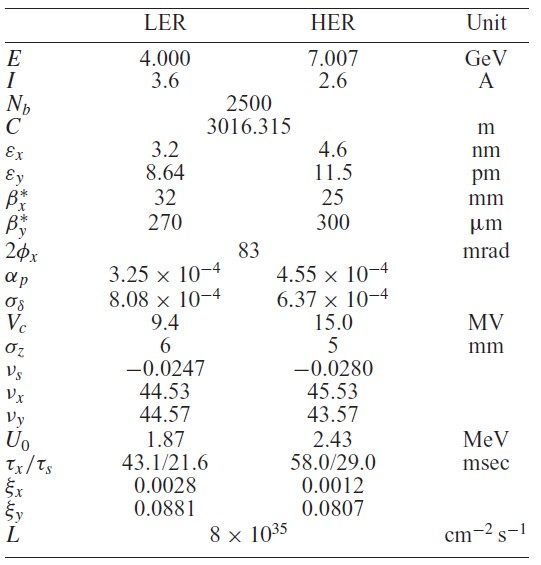
\includegraphics[scale=.6]{beam_par}
\caption{Machine parameters of SuperKEKB. The mark ''*'' indicate values in the IP.}
\label{fig:beampar}
\end{figure}
\end{comment}


%---------------------------------------------
%			1.3
%---------------------------------------------
\section{Belle II detector}


The Belle II detector is a general-purpose spectrometer which consists of a nested subdetectors sequence placed around the berillium beam pipe of 10 mm radius, nearby the IP of the two beams. Here we will go trough a briefly description of the several subdetectors (\autoref{fig:belle_detector}) going in order from the beam pipe outwards: the Vertex Detectors, the Central Drift Chamber, the TOP and the ARICH, the electromagnetic calorimeter and the $K_{L}$ muon detector.

\begin{figure}[h!]
\centering
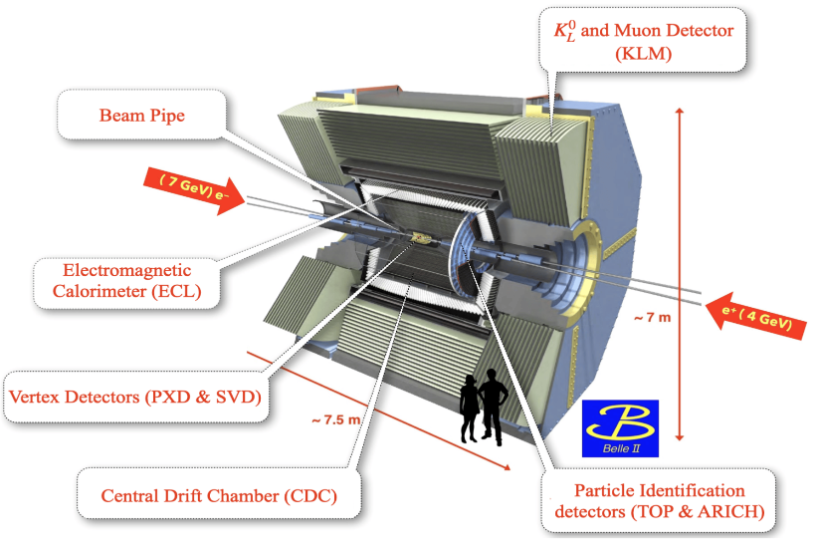
\includegraphics[scale=.8]{belle_detector}
\caption{Belle II detector.}
\label{fig:belle_detector}
\end{figure}


\subsection{Vertex Detectors (VXD)}


The \textbf{VerteX Detector (VXD)} is composed by two devices divided into layers, the silicon Pixel Detector (PXD) and the Silicon Vertex Detector (SVD), for a total of six layers around the beam pipe.\\
The inner two layers of PXD (L12) consist of pixelated sensors based on the depleted field effect transistor (DEPFET) techonology, realised with very thin (< 100 $\mu$m) sensors which allows to minimise multiple scattering, thus improving the tracking resolution for low-momentum particles. They are at a radius of 14 mm and 22 mm, respectively. \\
The remaining four layers of SVD (L3456) instead, are equipped with double-sided silicon strip (DSSD) sensors (at 39 mm, 80 mm, 104 mm and 135 mm respectively). Since a lower background rate is expected with respect to PXD, DSSD allow to achieve similar performance with a much smaller number of readout channels.
These layers are mainly used for tracking/vertexing and also for particle identification (PID), through the measurement of the energy loss (dE/dx).\\

We can notice in~\autoref{fig:VXD} that because of the essential asymmetric configuration of the beam energies and the consequent boost of the particles produced in the collisions (\autoref{sec:vertex_decay}), the structure of the vertex detectors is also asymmetric along the logitudinal axis.

\begin{figure}[h!]
\centering
\subfigure{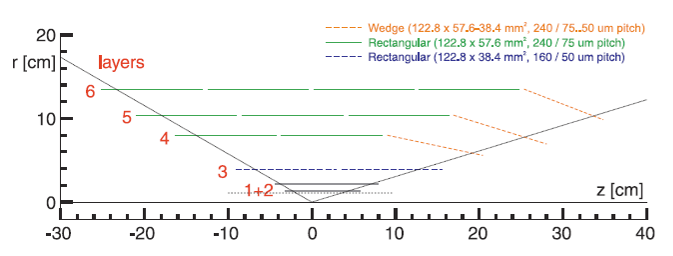
\includegraphics[scale=0.9]{VXD1}}\quad
\subfigure{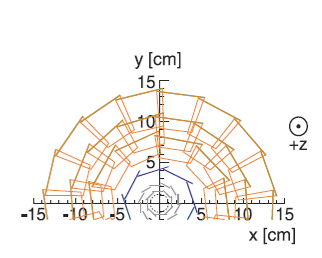
\includegraphics[scale=0.8]{VXD2}}\\
\caption{A schematic view of the Belle II vertex detector with a Be beam pipe and the six layers of PXD and SVD.}
\label{fig:VXD}
\end{figure}


\subsection{Central Drift Chamber (CDC)}

This is the central tracking device, with a large-volume drift chamber and small drift cells. The chamber gas is composed of a \ch{He-C_{2}H_{6}} (50:50) mixture with an average drift velocity of 3.3 \unit{\centi\meter.\micro\second^{-1}} and a maximum drift time of about 350 ns for a 17 mm cell size.\\
The CDC contains 14336 wires arranged in 56 layers either in \emph{axial}  (aligned with the solenoidal magnetic field) or \emph{stereo} (skewed with respect to the axial wires) orientation (\autoref{fig:CDC}). 
In fact by combining information from both the axial and the stereo layers it is possible to reconstruct full three-dimensional helix charged tracks and measure their momenta.
It also provides information for PID by measuring ionization energy loss, which is particularly useful for low-momentum particles that cannot reach the outer subdetectors dedicated also to deal with PID.

\begin{figure}[h!]
\centering
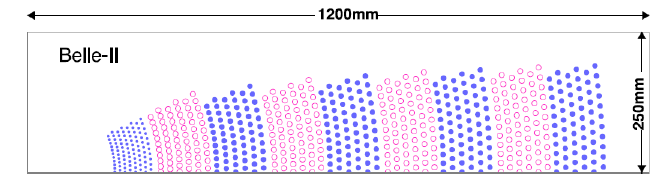
\includegraphics[scale=.9]{CDC}
\caption{Schematic view of the CDC drift cells: blue dots represent the axial wires and the pink empty ones the stereo wires.}
\label{fig:CDC}
\end{figure}


\subsection{Particle identification system (TOP e ARICH)}

\textbf{TOP (Time Of Propagation)} is a special kind of Cherenkov detector used for PID in the barrel region. It employs the two-dimensional information of a Cherenkov ring image, such as the time of arrival and the impact position of Cherenkov photons at the photodetector at one end of a 2.6 m quartz bar. It is composed by 16 detector modules, each one consisted in a \numproduct{45 x 2} cm quartz bar (Cherenkov radiator) with a small expansion volume (about 10 cm long) at the sensor end of the bar (\autoref{fig:TOP}). 

In order to achieve a single-photon time resolution of about 100 ps (required for a good PID), 16-channel of microchannel plate photomultiplier tubes (MCP-PMT) are employed, specially developed for this purpose.\\

\begin{figure}[h!]
\centering
\subfigure[A schematic view of the TOP radiator.]{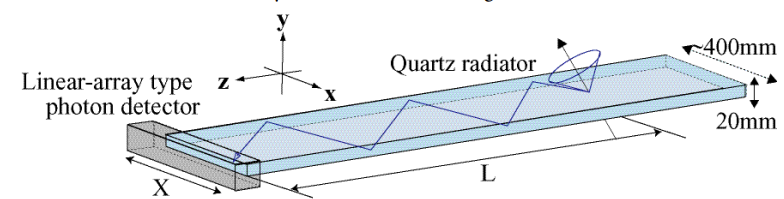
\includegraphics[scale=0.6]{TOP_quartz_radiator}}\\
\subfigure[A side view of the TOP radiator.]{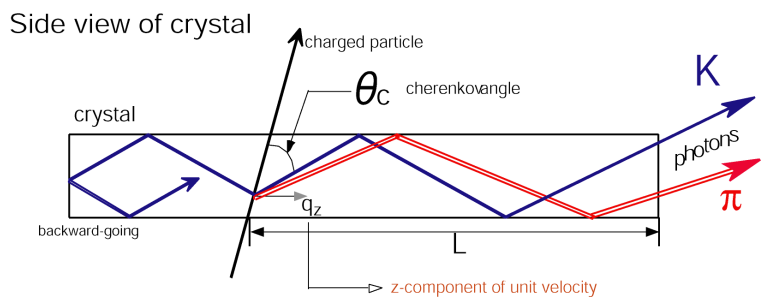
\includegraphics[scale=0.6]{TOP_side_view}}\\
\caption{TOP detector.}
\label{fig:TOP}
\end{figure}

\textbf{ARICH (Aerogel Ring Imaging CHerenkov)} is used to identify charged particles and it is placed in the forward endcap region. It is a proximity focusing Cherenkov ring-imaging detector which adopts aerogel as Cherenkov radiator. In particular this detector employs a novel method to increase the number of detected Cherenkov photons: two 2 cm-thock layers of aerogel with different refractive indices ($n_{1}$ = 1.045 upstream, $n_{2}$= 1.055 downstream) that increase the yield without degrading the Cherenkov angle resolution (\autoref{fig:ARICH}).

A hybrid avalanche photon detector (HAPD) are exploited as single-photon-sensitive high-granularity sensor. Here photo-electrons are accelerated over a potential difference of about 8 KV and are detected in avalanches photodiodes (APD).\\

\begin{figure}[h!]
\centering
\subfigure{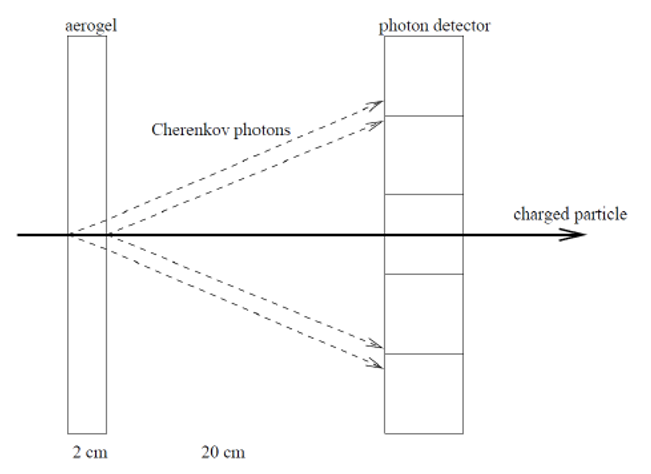
\includegraphics[scale=0.5]{ARICH1}}\quad
\subfigure{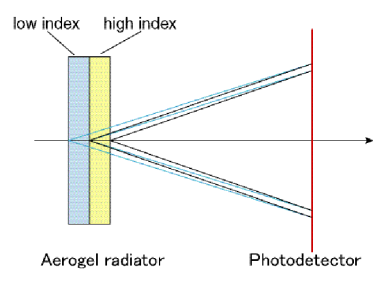
\includegraphics[scale=0.85]{ARICH2}}\\
\caption{ARICH detector.}
\label{fig:ARICH}
\end{figure}

The main task of these detectors is to improve the K/$\pi$ separation until 3.5 and 4 GeV/c of momentum, respectively.

\subsection{Electromagnetic calorimeter (ECL)}

The \textbf{ECL} is a highly segmented array of tallium-doped caesium iodide CsI(Tl) crystals assembled in a 3 m long barrel section with a radius of 1.25m, and two endcaps discs located at 2 m (forward) and 1 m (backward). All of them are instrumented with a total of 8736 crystal, covering about 90\% of the solid angle in center-of-mass system. 

This detector is used to detect gamma rays and to identify electrons in order to separate the latter from hadrons, expecially pions.

\subsection{$K_{L}$ muon detector (KLM)}

It consists of an alternating sandwich of 4.7 cm-thick iron plates and active detector elements located outside the volume of the superconducting solenoid that provides a 1.5 T magnetic field. The iron plates serve as the magnetic flux return joke for the solenoid. They also provide 3.9 interaction lenghts or more of material, beyond the 0.8 interaction lenghts of the calorimeter in which $K_{L}^{0}$ mesons can shower hadronically. The active detector elements have been chosen in order to cope with the reduction of the detector efficiency under the SuperKEKB background rates: resistive plate chambers (RPCs) for the outermost active layers and in the two innermost layers of the barrel and endcaps regions, scintillator strips with wavelenght-shifting fibers are used, readout by silicon photomultipliers (SiPMs).\\

In~\autoref{fig:detector_summary} a summary of the main characteristics of all subdetectors.


\begin{figure}[h!]
\centering
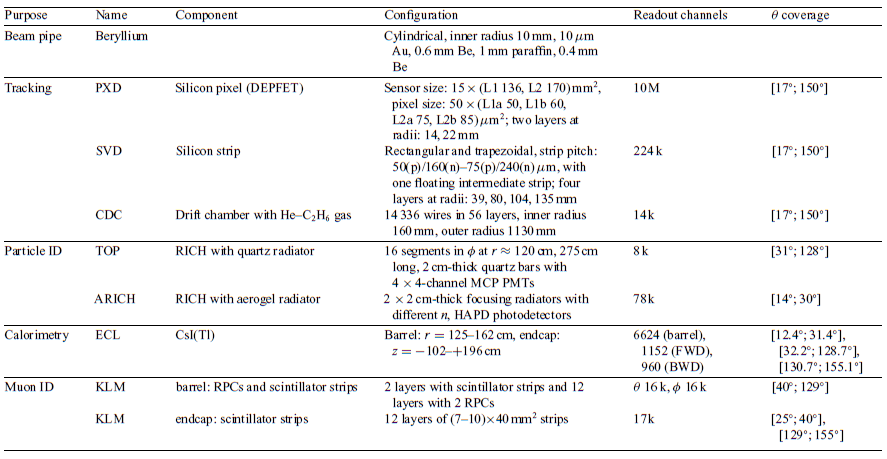
\includegraphics[width=12cm, height=7cm]{detector_summary}
\caption{Summary of the main characteristics of all subdetectors.}
\label{fig:detector_summary}
\end{figure}

\subsection{Trigger system}

The trigger system of Belle II has a non-trivial role to identify events of interest during data-taking at SuperKEKB, where high background rates are expected. 
This system is divided into two levels: a hardware-based low-level trigger (L1) and a software-based high-level trigger (HLT), implemented in the data acquisition (DAQ) system. 

\begin{itemize}
\item \textbf{L1}: has a latency of 5 $\mu$s and a maximum trigger output rate of 30 kHz, limited by the read-in rate of the DAQ.
\item \textbf{HLT}: is a key component of the DAQ, used to fully reconstruct events that pass the L1 trigger selection. It has to reduce online event rates to 10 kHz for offline storage and it must identify track regions of interest for PXD readout in order to reduce data flux. It fully recreates events with offline reconstruction algorithms, using all detectors infromation except for the PXD.
\end{itemize}



%---------------------------------------------
%			1.4
%---------------------------------------------
\section{Current state of data taking} \label{sec:perspectives}

SuperKEKB accelerator reaches a new luminosity peak of \num{4.7e34} $cm^{-2}s^{-1}$ in July 2022 (\autoref{fig:total_luminosity}).

\begin{figure}[h!]
\centering
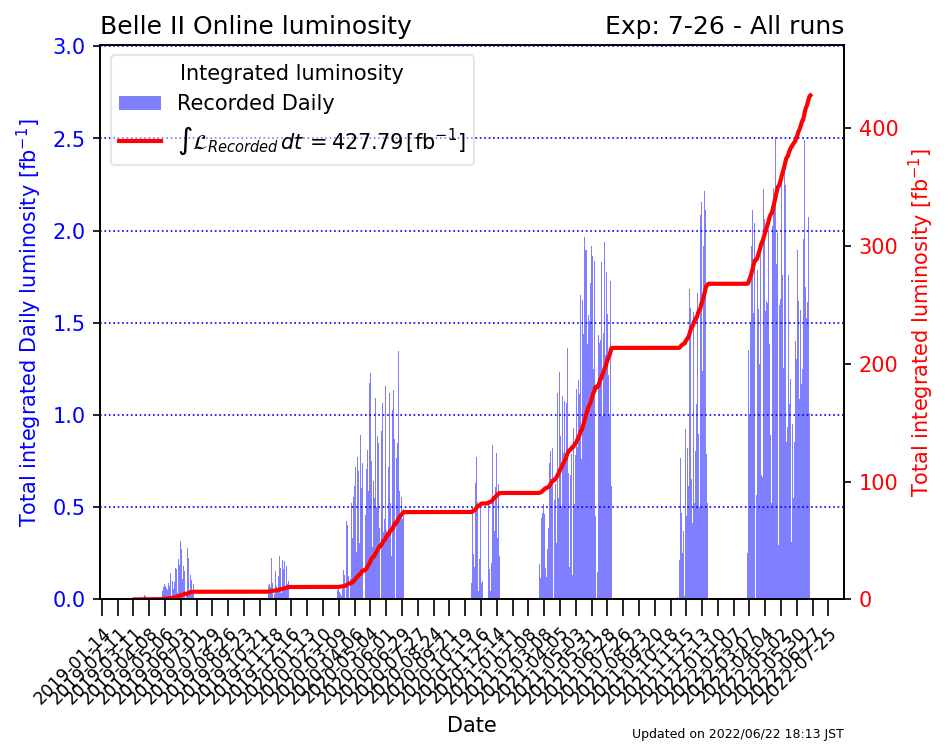
\includegraphics[scale=.6]{daily_luminosity}
\caption{Total recorded integrated luminosity before Long Shutdown 1.}
\label{fig:total_luminosity}
\end{figure}

In further perspectives, the target of SuperKEKB is to achieve a new record with \textit{$L_{ist}$} = \num{6e35} $cm^{-2}s^{-1}$ and to increase the integrated luminosity from 428 $fb^{-1}$ (current value, starting in 2019) to 50 $fb^{-1}$ (projection plot shown in~\autoref{fig:lumy_projection}), in order to increase the statistics and as consequence the hope to give an insight in some of the questions still open in the SM.\\

\begin{figure}
\centering
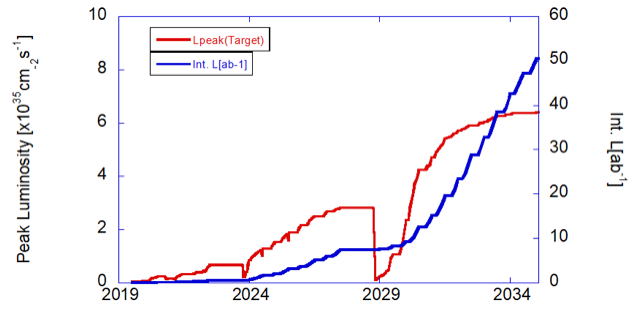
\includegraphics[scale=.7]{lumi_project}
\caption{Luminosity projection plot (plan for the coming years).}
\label{fig:lumy_projection}
\end{figure}

To accomplish the fixed goals mentioned above, an upgrade not only of the vertex detector but also of the whole experiment and of the interaction region is necessary, among several reasons, to cope with a more complex circumstances due to the increased luminosity which undermine its proper functioning.

Therefore a three-phase program has been drawn up:

\begin{itemize}
\item \textbf{short term}: year 2022. Long Shutdown 1 (LS1) is planned for approximately 15 months starting in July 2022, in order to install a complete pixel detector (PXD).
\item \textbf{medium term}: approximately year 2028-29. Long Shutdown 2 (LS2) will probably be needed for the upgrade of the Interaction Region (IR) to reach a new luminosity target $\textit{L}_{peak}$ = \num{6e35} $cm^{-2}s^{-1}$. 
Several open questions and difficulties have triggered many studies and discussions about a possible redesign of the machine lattice during this phase. In particular it would be necessary to deal with the limitation of the optics of the machine, concerning the further increasing of the luminosity and accordingly of the backgrounds rates. A new Vertex Detector might be also required, to accommodate the new IR design, and other sub-detector upgrades are possible. 
\item \textbf{long term}: years > 2032. Studies have started to explore upgrades beyond the currently planned program, such as beam polarization and ultra-high luminosity and so possibly $\textit{L}_{peak}$ in excess of \num{1e36} $cm^{-2}s^{-1}$. While the beam polarization has a concrete proposal, for ultra-high luminosity studies have just started.
\end{itemize}

At time of writing we are in the period of a long shut-down (LS1), last since June 2022 and the installation of a complete pixel detector (PXD) is almost done. The restart of data taking is planned at the beginning of 2024.

